% !TEX root = ./F1-Exercicios_Resoluções.1.tex
\providecommand\mainfilename{"./F1-Exercicios_Resoluções.tex"}
\providecommand \subfilename{}
\renewcommand   \subfilename{"./F1-Exercicios_Resoluções.1.tex"}
\documentclass[\mainfilename]{subfiles}

% \tikzset{external/force remake=true} % - remake all

\begin{document}

\graphicspath{{\subfix{./.build/figures/F1-Exercicios_Resoluções.1/}}}
\tikzsetexternalprefix{./.build/figures/F1-Exercicios_Resoluções.1/}

\mymakesubfile{1}
[Física 1]
{Exercicios Resoluções: Vetores} % Subfile Title
{Vetores} % Part Title

\begin{questionBox}1{ % Q1
    Dado o vector \(\vv{A}\) da figura seguinte, desenhe os vectores \(\frac{1}{2}\vv{A}\) e \(2\,\vv{A}\)
} % Q1
    \answer{}
    % \tikzset{external/remake next=true}
    \begin{center}
        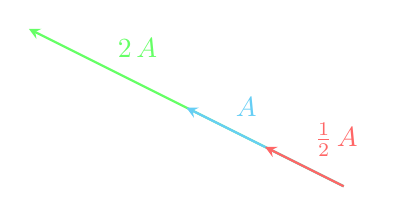
\begin{tikzpicture}
    
            \draw[-stealth,thick,green!60!]
            ( 0,0) --
            (-2,1) --node[above right]{\(2\,A\)}
            (-4,2);
            
            \draw[-stealth,thick,cyan!60!]
            ( 0,0  )--
            (-1,0.5)--node[above right]{\(A\)}
            (-2,1  );
            
            \draw[-stealth,thick,red!60!]
            ( 0,0  )--node[anchor=south west]{\(\frac{1}{2}\,A\)} 
            (-1,0.5);
        
        \end{tikzpicture}
    \end{center}
\end{questionBox}

\begin{questionBox}1{ % Q2
    Para cada um dos pares de vetores \(\vv{A}\) e \(\vv{B}\) seguintes, obtenha graficamente o vector diferença \(\vv{A}-\vv{B}\)
} % Q2
    \answer{}
    \begin{multicols}{2}

        \begin{questionBox}2{} % Q2.1
            % \tikzset{external/remake next=true}
            \begin{center}
            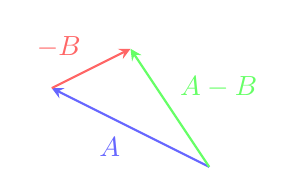
\begin{tikzpicture}
            
                \draw[-stealth, thick, blue!60!]
                ( 0,0)--node[anchor=north east]{\(\vv{A}\)}
                (-2,1);
                
                \draw[-stealth, thick, red!60!]
                (-2,1  )--node[anchor=south east]{\(-\vv{B}\)} 
                +( 1,0.5);
                
                \draw[stealth-, thick, green!60!]
                (-1,1.5)
                --node[anchor=south west]{\(\vv{A}-\vv{B}\)}
                ( 0,0  );
                
            \end{tikzpicture}
            \end{center}
        \end{questionBox}

        \begin{questionBox}2{} % Q2.2
            \begin{center}
            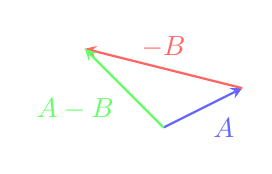
\begin{tikzpicture}
	
                \draw[-stealth, thick, blue!60!] 
                (0,0  )
                --node[anchor=north west]{\(\vv{A}\)}
                (1,0.5);
                
                \draw[-stealth, thick, red!60!]
                ( 1,0.5)
                --node[anchor=south]{\(-\vv{B}\)}
                +(-2,0.5);
                
                \draw[stealth-, thick, green!60!]
                (-1,1)
                --node[anchor=north east]{\(\vv{A}-\vv{B}\)}
                ( 0,0);
                
            \end{tikzpicture}
            \end{center}
        \end{questionBox}

        \begin{questionBox}2{} % Q2.3
            \begin{center}
            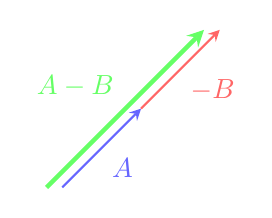
\begin{tikzpicture}
                
                \draw[-stealth, thick, blue!60!]
                (0,0)
                --node[anchor=north west]{\(\vv{A}\)}
                (1,1);
                
                \draw[-stealth, thick, red!60!]
                (1,1)
                --node[anchor=north west]{\(-\vv{B}\)}
                +(1,1);

                \draw[-stealth, ultra thick, green!60!]
                (-0.2,0)
                --node[anchor=south east]{\(\vv{A}-\vv{B}\)}
                ( 1.8,2);
                
            \end{tikzpicture}
            \end{center}
        \end{questionBox}

    \end{multicols}
\end{questionBox}

\begin{questionBox}1{ % Q3
    Dados os vectores \(\vv{A}\text{ e }\vv{B}\) seguintes, obtenha graficamente o vector \(\vv{C}=2\,\vv{A}-3\,\vv{B}\).
} % Q3
    \answer{}
    \begin{center}
    % \tikzset{external/remake next=true}
    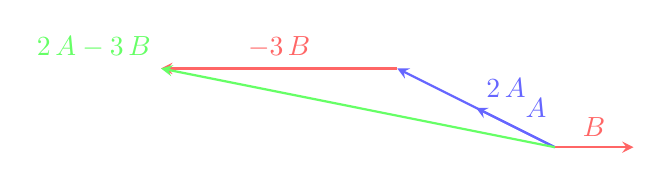
\begin{tikzpicture}

        \draw[-stealth, thick, blue!60!]
        ( 0,  0)
        --node[anchor=south west]{\(\vv{A}\)}
        (-1,0.5);
        
        \draw[-stealth, thick, blue!60!]
        ( 0,0  )
        --node[anchor=south west]{\(2\,\vv{A}\)}
        (-2,1  );
        
        \draw[-stealth, thick, red!60!]
        (0,0)
        --node[anchor=south]{\(\vv{B}\)}
        (1,0);
        
        \draw[-stealth, thick, red!60!]
        (-2,1)
        --node[anchor=south]{\(-3\,\vv{B}\)}
        +(-3,0);
        
        \draw[-stealth, thick, green!60!]
        ( 0,0)
        --(-5,1) 
        node[anchor=south east]{\(2\,\vv{A}-3\,\vv{B}\)};
        
    \end{tikzpicture}
    \end{center}
\end{questionBox}

\begin{questionBox}1{ % Q4
    Obtenha os valores numéricos das componentes (escalares), segundo os eixos dos \textit{x} e dos \textit{y}, de cada um dos vectores indicados.
} % Q4
    \answer{}
    \begin{questionBox}2{} % Q4.1
        \begin{flalign*}
            &
                \vv{A}
                = 5\,\cos(130^\circ)\,\hat{\imath}
                + 5\,\sin(130^\circ)\,\hat{\jmath}
                \cong -3.2\,\hat{\imath}+3.8\,\hat{\jmath}
            &
        \end{flalign*}
    \end{questionBox}

    \begin{questionBox}2{} % Q4.2
        \begin{flalign*}
            &
                \vv{B}
                = -4\,\cos(30^\circ)\,\hat{\imath}
                -4\,\sin(30^\circ)\,\hat{\jmath}
                = -2\sqrt{3}\,\hat{\imath}
                - 2\,\hat{\jmath}
            &
        \end{flalign*}
    \end{questionBox}

    \begin{questionBox}2{} % Q4.2
        \begin{flalign*}
            &
                \vv{C}
                = 5\,\cos(45^\circ)\,\hat{\imath}
                - 5\,\sin(45^\circ)\,\hat{\jmath}
                = \frac{5\sqrt{2}}{2}\hat{\imath}
                - \frac{5\sqrt{2}}{2}\hat{\jmath}
            &
        \end{flalign*}
    \end{questionBox}
\end{questionBox}

\begin{questionBox}1{ % Q5
    Quais são as componentes, segundo os eixos dos \textit{x} e dos \textit{y}, do vector soma \(\vv{D}=\vv{A}+\vv{B}+\vv{C}\) dos três vectores referidos na questão Q4?
} % Q5
    \answer{}
    \begin{flalign*}
        &
            \vec D 
            = \vv{A}+\vv{B}+\vv{C}
            \cong 
            (-3.2-2\sqrt{3}+5\sqrt{2}/2)\hat{\imath}
            + (3.8 - 2 - 5\sqrt{2}/2)\hat{\jmath}
            \cong 
            -3.1\,\hat{\imath}
            -1.7\,\hat{\jmath}
        &
    \end{flalign*}
\end{questionBox}

\begin{questionBox}1{ % Q6
    Um vector pode ter uma componente nula e módulo não nulo? Justifique.
} % Q6
    \answer{}
    Sim,
    \begin{flalign*}
        &
            \{
                \forall\, V\subset\mathbb{R}^n: v_i= 0;
                i\in\mathbb{N}
            \}
            \implies \sum_{k=1}^{n}{v_k^2} \geq 0 
            \implies \myvert{\vv{V}}\geq 0 
        &
    \end{flalign*}
\end{questionBox}

\begin{questionBox}1{ % Q7
    Um vector pode ter módulo nulo e uma componente não nula? Justifique.
} % Q7
    \answer{}
    Não,
    \begin{flalign*}
        &
            \{ 
                \forall\, V\subset\mathbb{R}^n : v_i \neq 0;
                i\in\mathbb{N}
            \}
            \implies \sum_{k=1}^{n}{v_k^2} > 0 
            \implies \myvert{\vv{V}}> 0
        &
        \end{flalign*}
\end{questionBox}

\begin{questionBox}1{ % Q8
    Para cada vector cujas componentes segundo os eixos dos \textit{x} e dos \textit{y} são indicadas:
} % Q8
    \begin{itemize}
        \item Desenhe o vector utilizando o sistema de eixos apresentado;
        \item Indique o ângulo \(\theta\) que define a direcção e sentido do vector;
        \item Obtenha o módulo do vector e o valor de \(\theta\).
    \end{itemize}

    \subquestion{\(A_x=\phantom{+}3,A_y=-2\)}
    \subquestion{\(B_x=-2,B_y=\phantom{+}2\)}
    \subquestion{\(C_x=\phantom{+}0,C_y=-2\)}

    \answer{}

    % \tikzset{external/remake next=true}
    \begin{center}
    \begin{tikzpicture}
        % [ scale=0.7, font={\fontsize{8}{0}} ]

        \coordinate (x) at ( 4, 0);
        \coordinate (y) at ( 0, 3);
        \coordinate (0) at ( 0, 0);
        \coordinate (a) at ( 3,-2);
        \coordinate (b) at (-2, 2);
        \coordinate (c) at ( 0,-2);
        
        \draw[ultra thin, black!60!] (-3,-3) grid (4,3);
        
        \draw[->] (-3, 0)--(x) node[right]{\textit{x}};
        \draw[->] ( 0,-3)--(y) node[above]{\textit{y}};
        
        \draw[->, green!60!](0)--(a) node[right]{\textit{A}};
        \draw[->, cyan!60!] (0)--(b) node[above]{\textit{B}};
        \draw[->, red!60!]  (0)--(c) node[below right]{\textit{C}};
        
        \draw pic[
            pic text=\(-33.7^\circ\),
            draw=green!40!,
            text=green!40!,
            <-,
            angle eccentricity=2, 
            angle radius=0.7cm
        ] { angle=a--0--x };
        
        \draw pic[
            pic text=\(45^\circ\),
            draw=cyan!40!,
            text=cyan!40!,
            ->,
            angle eccentricity=1.5,
            angle radius=0.6cm
        ] { angle=x--0--b };
        
        \draw pic[
            draw=red!40!,
            text=red!40!,
            ->,
            angle eccentricity=2,
            angle radius=0.4cm
        ] { angle=x--0--c };
        
        \node[text=red!40!] at (-0.9,-0.6){\(\pi\frac{3}{2}\)};
        
    \end{tikzpicture}
    \end{center}
\end{questionBox}

\begin{questionBox}1{ % Q9
    Dado o vector \(\vv{A}(5, 30^\circ\text{ (acima da horizontal)})\) , obtenha as componentes \(A_x\) e \(A_y\) nos três sistemas de coordenadas indicados abaixo.
} % Q9
    \answer{}
    \begin{questionBox}2{} % Q9.1
        \begin{flalign*}
            &	
                \vec A 
                = 5\,\cos(30^\circ)\,\hat{\imath}
                + 5\,\sin(30^\circ)\,\hat{\jmath}
                = 2.5\sqrt{3}\,\hat{\imath}
                + 2.5\,\hat{\jmath}
            &
        \end{flalign*}

        % \tikzset{external/remake next=true}
        \begin{center}
        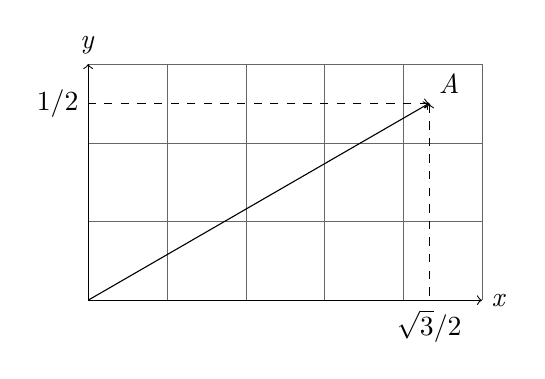
\begin{tikzpicture}
        
            \coordinate (0) at (0,0);
            \coordinate (x) at (5,0);
            \coordinate (y) at (0,3);
            \coordinate (a) at (30:5);
            
            \draw[ultra thin, black!60!] (0) grid +(y) grid +(x);
            
            \draw[<->] 
            (y)
            node[above]{\textit{y}}
            --(0)--(x)
            node[right]{\textit{x}};
            
            \draw[->] (0) -- (a) node[above right]{\textit{A}};
            
            \draw[<-, thin, dashed]
            (a) -- (a |- 0,0)
            node[below]{\(\sqrt{3}/2\)};

            \draw[<-, thin, dashed]
            (a) -- (0,0 |- a)
            node[left]{\(1/2\)};
        
        \end{tikzpicture}
        \end{center}
    \end{questionBox}

    \begin{questionBox}2{} % Q9.2
        \begin{flalign*}
            &	
                \vv{A}=5\,\cos(60^\circ)\,\hat{\imath}
                + 5\,\sin(60^\circ)\,\hat{\jmath}
                = 2.5\,\hat{\imath}
                + 2.5\sqrt{3}\,\hat{\jmath}
            &
        \end{flalign*}

        \begin{center}
        \begin{tikzpicture}[rotate=-30]
        
            \coordinate (0) at (0,0);
            \coordinate (x) at (4,0);
            \coordinate (y) at (0,5);
            \coordinate (a) at (60:5);
            
            \draw[ultra thin, black!60!] (0) grid +(y) grid +(x);
            
            \draw[<->]
            (y) 
            node[above]{\textit{y}}
            --(0)--(x) 
            node[right]{\textit{x}};
            
            \draw[->,thick]
            (0) -- (a) node[above right]{\textit{A}};
            
            \draw (0) -- (30:4) coordinate(b)
            pic[
                pic text=\(30^\circ\), 
                draw, 
                angle eccentricity = 1.5, 
                angle radius = 1cm
            ] {angle=x--0--b}
            pic[
                pic text=\(30^\circ\), 
                draw, 
                angle eccentricity = 1.5, 
                angle radius = 1.2cm
            ] {angle=b--0--a};
            
            \draw[<-, thin, dashed] 
            (a) -- (a |- 0,0) node[below]{\(2.5\)};
            \draw[<-, thin, dashed] 
            (a) -- (0,0 |- a) node[left]{\(2.5\sqrt{3}\)};
        
        \end{tikzpicture}
        \end{center}
    \end{questionBox}

    \begin{questionBox}2{} % Q9.3
        \begin{flalign*}
            &
                \vv{A}
                = 5\,\cos(-15^\circ)\,\hat{\imath}
                + 5\,\sin(-15^\circ)\,\hat{\jmath}
                \cong
                \num{4.829629131445341}\,\hat{\imath}
                - \num{1.294095225512604}\,\hat{\jmath}
            &
        \end{flalign*}

        % \tikzset{external/remake next=true}
        % \begin{center}
        % \begin{tikzpicture}[rotate=45]

        %     \coordinate (0) at (0,0);
        %     \coordinate (x) at (5,0);
        %     \coordinate (y) at (0,-2);
            
        %     \draw[ultra thin, black!60!] (0,-2) grid (x);
            
        %     \draw[<->] 
        %     (y) 
        %     node[above]{\(-y\)}
        %     --(0)--(x)
        %     node[right]{\textit{x}};
            
        %     \draw[->,thick]
        %     (0) -- (-15:5)
        %     coordinate(a)
        %     node[above right]{\textit{A}};

        % 	\draw 
        %     (0) -- (30:4) 
        %     coordinate(b)
        % 	pic[
        %         pic text=\(30^\circ\), 
        %         draw, 
        %         angle eccentricity = 1.5, 
        %         angle radius = 1cm
        %     ] {angle=x--0--b}
        % 	pic[
        %         pic text=\(30^\circ\), 
        %         draw, 
        %         angle eccentricity = 1.5, 
        %         angle radius = 1.2cm
        %     ] {angle=b--0--a};
        	
        % 	% \draw[<-, thin, dashed] 
        %     % (a) -- (a |- 0,0) node[below]{\(2.5\)};

        % 	% \draw[<-, thin, dashed] 
        %     % (a) -- (0,0 |- a) node[left]{\(2.5\sqrt{3}\)};
        
        % \end{tikzpicture}
        % \end{center}
    \end{questionBox}
\end{questionBox}

\renewcommand\thequestion{Problema \arabic{question}}
\renewcommand\thesubquestion{P\arabic{question} \alph{subquestion}.}

\begin{minipage}{1\textwidth}
    \group{}
    
    Nestes problemas, os vectores unitários que definem a direcção e sentido dos eixos coordenados \textit{x,y,z} são denominados, respectivamente, por \(\hat{\imath},\hat{\jmath},\hat{k}\).
\end{minipage}

\begin{questionBox}1{ % P1
    Calcule:
} % P1
    \begin{questionBox}2{ % P1.1
        O módulo do vetor \(\vv{a}=\hat{\imath}+2\,\hat{\jmath}+2\,\hat{k}\)
    } % P1.1
        \answer{}
        \begin{flalign*}
            &
                \myvert{\vv{a}}
                =\sqrt{1+2^2+2^2}
                = 3
            &
        \end{flalign*}
    \end{questionBox}

    \begin{questionBox}2{ % P1.2
        O vector unitário com a direcção e sentido de \(\vv{a}\) (Dado um vector \(\vv{a}\), o vector unitário com a
        direcção e sentido de \(\vv{a}\), que poderemos denotar por \(\hat{a}\), denomina-se versor de \(\vv{a}\)).
    } % P1.2
        \answer{}
        \begin{flalign*}
            &
                \hat{a}
                = \frac{\vv{a}}{\myvert{\vv{a}}}
                = 3^{-1}\,\hat{\imath}
                + 1.5^{-1}\,\hat{\jmath}
                + 1.5^{-1}\,\hat{k}
            &
        \end{flalign*}
    \end{questionBox}
\end{questionBox}

\begin{questionBox}1{ % P2
    Dados os vectores \(\vv{a}\) e \(\vv{b}\), cujas componentes segundo os eixos coordenados \textit{x}, \textit{y} e \textit{z} são, respectivamente
} % P2
    \begin{BM}[align*]
        a_x = 5; & a_y = 4; & a_z=-3
        \\
        b_x = 3; & b_y =-4; & b_z=5
    \end{BM}

    \begin{questionBox}2{ % P2.1
        O vetor \(\vv{c}=6\,\vv{a}-3\,\vv{b}\)
    } % P2.1
        \answer{}
        \begin{flalign*}
            &
                \vv{c}
                = (30-9)\hat{\imath}
                + (24+12)\hat{\jmath}
                + (-18-15)\hat{k}
                = 21\,\hat{\imath}
                + 36\,\hat{\jmath}
                - 33\,\hat{k}
            &
        \end{flalign*}
    \end{questionBox}

    \begin{questionBox}2{ % P2.2
        A quantidade \(\vv{a}^2+\vv{b}^2\)
    } % P2.2
        \answer{}
        \begin{flalign*}
            &
                \vec a^2+\vec b^2
                = 25+16+9+9+16+25
                =100
            &
        \end{flalign*}
    \end{questionBox}

    \begin{questionBox}2{ % P2.3
        O ângulo entre os vetores \(\vv{a}\text{ e }\vv{b}\)
    } % P2.3
        \answer{}
        \begin{flalign*}
            &
                \myvert{\vv{a}}\,\myvert{\vv{b}}\,\cos(\theta)
                = a_x\,b_x
                + a_y\,b_y
                + a_z\,b_z
                \implies &\\&
                \implies
                \theta
                =\arccos\left( 
                    \frac{15-16-15}{\sqrt{50}\,\sqrt{50}} 
                \right)
                \cong 108.66^\circ
            &
        \end{flalign*}
    \end{questionBox}

    \begin{questionBox}2{ % P2.4
        A projeção de \(\vv{b}\) segundo \(\vv{a}\)
    } % P2.4
        \answer{}
        \begin{flalign*}
            &
                \myvert{\vv{b}}\,\cos(\theta)\,\hat{a}
                = \sqrt{50}\,\cos(108.66^\circ)\,\hat{a}
                \cong -2.26\,\hat{a}
            &
        \end{flalign*}
    \end{questionBox}
\end{questionBox}

\begin{questionBox}1{ % P3
    Dados os pontos \(P(x_1,y_1,z_1)\text{ e }Q(x_2,y_2,z_2)\), escreva a expressão cartesiana (isto é, em termos dos vectores unitários segundo os eixos dos \textit{x}, \textit{y} e \textit{z}) do vector \(\vv{P\,Q}\) e obtenha a expressão do seu módulo.
} % P3
    \answer{}
    \begin{flalign*}
        &
            \vv{P\,Q}
            =\vec Q-\vec P 
            = (x_2-x_1)\hat{\imath}
            + (y_2-y_1)\hat{\jmath}
            + (z_2-z_1)\hat{k}
            = &\\&
            = \sqrt{(x_2-x_1)^2+(y_2-y_1)^2+(z_2-z_1)^1}
        &
    \end{flalign*}
\end{questionBox}

\begin{questionBox}1{ % P4
    Considere os dois vectores \(\vv{u}\text{ e }\vv{v}\), no plano \(x\,0\,y\), possuindo, respectivamente, os módulos \(\sqrt{3}\) e 1. O vector \(\vv{u}\) faz com o semi-eixo \(0\,x\) um ângulo de \(30^\circ\) e o vector \(\vv{v}\) faz com esse semi-eixo um ângulo de \(60^\circ\). Calcule:
} % P4
    \begin{questionBox}2{ % P4.1
        As componentes \(\vv{u}\text{ e }\vv{v}\), segundo os eixos dos \textit{x}, \textit{y} e \textit{z}
    } % P4.1
        \answer{}
        \begin{flalign*}
            &
                \vv{u}
                = \sqrt{3}\,\cos(30^\circ)\,\hat{\imath}
                + \sqrt{3}\,\sin(30^\circ)\,\hat{\jmath}
                + 0\,\hat{k}
                = 1.5\,\hat{\imath} 
                + \sqrt{3}/2\,\hat{\jmath}
                + 0\,\hat{k} 
            &\\&
                \vv{v}
                = \cos(60^\circ)\,\hat{\imath}
                + \sin(60^\circ)\,\hat{\jmath}
                + 0\,\hat{k}
                = 0.5\,\hat{\imath}
                + \sqrt{3}/2\,\hat{\jmath}
                + 0\,\hat{k}
            &
        \end{flalign*}
    \end{questionBox}

    \begin{questionBox}2{ % P4.2
        As componentes da resultante da adição de \(\vv{u}\text{ e }\vv{v}\)
    } % P4.2
        \answer{}
        \begin{flalign*}
            &
                \vv{u}+\vv{v} 
                = 2\,\hat{\imath}
                + \sqrt{3}\,\hat{\jmath}
                + 0\,\hat{k} 
            &
        \end{flalign*}
    \end{questionBox}

    \begin{questionBox}2{ % P4.3
        O módulo dessa resultante
    } % P4.3
        \answer{}
        \begin{flalign*}
            &
                \myvert{\vv{u}+\vv{v}}
                = \sqrt{2^2+\left(\sqrt{3}\right)^2+0^2}
                = \sqrt{7}
            &
        \end{flalign*}
    \end{questionBox}

    \begin{questionBox}2{ % P4.4
        As componentes do vetor diferença \(\vv{u}-\vv{v}\)
    } % P4.4
        \answer{}
        \begin{flalign*}
            &	
                \vv{u}-\vv{v} 
                = 1\,\hat{\imath}
                + 0\,\hat{\jmath}
                + 0\,\hat{k}
            &
        \end{flalign*}
    \end{questionBox}

    \begin{questionBox}2{ % P4.5
        O módulo do vetor \(\vv{u}-\vv{v}\)
    } % P4.5
        \answer{}
        \begin{flalign*}
            &
                \myvert{\vv{u}-\vv{v}}
                =1
            &
        \end{flalign*}
    \end{questionBox}

    \begin{questionBox}2{ % Q4.6
        O produto interno \(\vv{u}\cdot\vv{v}\)
    } % Q4.6
        \answer{}
        \begin{flalign*}
            &
                \vv{u}\cdot\vv{v} 
                = 1.5*0.5
                + \frac{\sqrt{3}}{2}
                * \frac{\sqrt{3}}{2}
                + 0*0
                = 0.75+0.75+0
                = 1.5
            &
        \end{flalign*}
    \end{questionBox}
\end{questionBox}

\begin{questionBox}1{ % P5
    Calcul o módulo do vetor \(\vv{r}=\vv{a}+\vv{b}+\vv{c}\), em que \(\vv{a},\vv{b}\text{ e }\vv{c}\) são os vetores abaixo indicados e o ângulo que o vector \(\vv{r}\) faz com o semi-eixo positivo dos \textit{x}.
} % P5

    \begin{BM}[align*]
        \vv{a}=(37;30^\circ)
        & \vv{b}=(25;60^\circ)
        & \vv{c}=(30;135^\circ)
    \end{BM}

    Aqui os vectores são denotados por \(\myvert{\vv{v}},\theta\), em que \(\myvert{\vv{v}}\) representa a amplitude do vector e \(\theta\) representa o ângulo que o vector faz com o semi-eixo positivo dos \textit{x}.

    \answer{}
    \begin{flalign*}
        & 
            \myvert{\vv{r}}
            = \myvert{\vv{a}+\vv{b}+\vv{c}}
            = \myvert{
                \begin{aligned}
                    &
                        (
                            37\,\cos(30^\circ)
                            &+& 25\,\cos(60^\circ)
                            &+& 30\,\cos(135^\circ)
                        )&\hat{\imath}
                    &+\\+&
                        (
                            37\,\sin(30^\circ)
                            &+& 25\,\sin(60^\circ)
                            &+& 30\,\sin(135^\circ)
                        )&\hat{\jmath}
                    &
                \end{aligned}
            }
            = &\\&
            = \myvert{
                \begin{aligned}
                    &
                        (18.5\sqrt3+12.5-15\sqrt2)&\hat{\imath}
                    &+\\+&
                        (18.5+12.5\sqrt3+15\sqrt2)&\hat{\jmath}
                    &
                \end{aligned}
            }
            \cong
            \myvert{
                23.33\,\hat{\imath}
                + 61.36\,\hat{\jmath}
            }
            \cong 65.65 
            &\\[3ex]&
            \theta_r 
            = \arccos(r_x/\myvert{\vv{r}})
            \cong \arccos(23.33/65.65)
            \cong 69.18^\circ
        &
    \end{flalign*}
\end{questionBox}

\begin{questionBox}1{ % P6
    Decomponha um deslocamento de 80\,\unit{\kilo\metre} numa direcção \(60^\circ\) para sul da direção \textbf{Este} em dois vectores, um dos quais na direcção \textbf{Este}.
} % P6
    \answer{}
    \begin{flalign*}
        &
            \vv{d}
            =(80\,\unit{\kilo\metre},-60^\circ)
            = 80\,\unit{\kilo\metre}\,\cos(60^\circ)\,\hat{e}
            - 80\,\unit{\kilo\metre}\,\sin(60^\circ)\,\hat{s}
            = 40\,\unit{\kilo\metre}\,\hat{e}
            - 40\,\sqrt{3}\,\hat{s} 
        &
    \end{flalign*}
\end{questionBox}

\begin{questionBox}1{ % P7
    Um barco parte do seu porto, tendo-se deslocado de 160\,\unit{\kilo\metre} para norte do ponto de partida. Decomponha o deslocamento do barco em dois vectores componentes, um dirigido para nordeste e o outro para noroeste. Que distância teria o barco percorrido a mais para atingir a sua posição final, se viajasse primeiramente para nordeste e depois para noroeste?
} % P7
    \answer{}
    \begin{flalign*}
        &	 
              \myvert{B_{ne}\hat{ne} }
            + \myvert{B_{nw}\hat{nw}}
            - \myvert{B_n\,\hat n}
            = 160\,(\cos(45^\circ) + \sin(45^\circ) - 1)
            \cong 66.27
        &
    \end{flalign*}
\end{questionBox}

\end{document}